% 独自のコマンド

% ■ アブストラクト
%  \begin{jabstract} 〜 \end{jabstract}  :日本語のアブストラクト
%  \begin{eabstract} 〜 \end{eabstract}  :英語のアブストラクト

% ■ 謝辞
%  \begin{acknowledgment} 〜 \end{acknowledgment}

\newif\ifjapanese

\japanesetrue  % 論文全体を日本語で書く(英語で書くならコメントアウト)

\ifjapanese
  \documentclass[a4j,twoside,openright,11pt]{jreport} % 両面印刷の場合。余白を綴じ側に作って右起こし。
  %\documentclass[a4j,11pt]{jreport}                  % 片面印刷の場合。
  \renewcommand{\bibname}{参考文献}
  \newcommand{\acknowledgmentname}{謝辞}
\else
  \documentclass[a4paper,11pt]{report}
  \newcommand{\acknowledgmentname}{Acknowledgment}
\fi
\usepackage[dvipdfmx]{graphicx}
\usepackage{thesis}
\usepackage{ascmac}
\usepackage{graphicx}
\usepackage{multirow}
\usepackage{url}
\usepackage{latexsym}
\usepackage{here}
\usepackage{listings,jlisting}

\lstset{%
  language={C},
  basicstyle={\small\ttfamily\footnotesize},%
  breaklines=true,%
  identifierstyle={\small},%
  commentstyle={\small\itshape},%
  keywordstyle={\small\bfseries},%
  ndkeywordstyle={\small},%
  stringstyle={\small\ttfamily},
  frame={tb},
  breaklines=true,
  columns=[l]{fullflexible},%
  numbers=left,%
  xrightmargin=0zw,%
  xleftmargin=3zw,%
  numberstyle={\scriptsize},%
  stepnumber=1,
  numbersep=1zw,%
  lineskip=-0.5ex%
}
\bibliographystyle{jplain}

\bindermode  % ファイル綴じ用余白設定

% 日本語情報(必要なら)
\jclass  {修士論文}                             % 論文種別
\jtitle  {手書きベースWikiシステムの研究}      % タイトル。改行する場合は\\を入れる
\juniv   {慶應義塾大学大学院}                   % 大学名
\jfaculty{政策・メディア研究科}                 % 学部、学科
\jauthor {早川 匠}                            % 著者
\jhyear  {元}                                   % 令和○年度
\jsyear  {2019}                                 % 西暦○年度
\jkeyword{手書きメモ、イラスト、Wiki、ハイパーテキスト、ユーザーインターフェース}       % 論文のキーワード
\jproject{} % プロジェクト名
\jdate   {2020年1月}

% 英語情報(必要なら)
\eclass  {Master's Thesis}                          % 論文種別
\etitle  {A study on drawing-based wiki systems}      % タイトル。改行する場合は\\を入れる
\euniv   {Keio University}                          % 大学名
\efaculty{Graduate School of Media and Governance}  % 学部、学科
\eauthor {Takumi Hayakawa}                                % 著者
\eyear   {2019}                                     % 西暦○年度
\ekeyword{Handwritten notes, illustration,Wiki, Hypertext, User Interface}          % 論文のキーワード
\eproject{}               % プロジェクト名
\edate   {January 2020}


\begin{document}

\ifjapanese
  \jmaketitle    % 表紙(日本語)
\else
  \emaketitle    % 表紙(英語)
\fi

% ■ アブストラクトの出力 ■
%	◆書式:
%		begin{jabstract}〜end{jabstract}	:日本語のアブストラクト
%		begin{eabstract}〜end{eabstract}	:英語のアブストラクト
%		※ 不要ならばコマンドごと消せば出力されない。



% 日本語のアブストラクト
\begin{jabstract}

 手書きメモやイラスト等のグラフィカルなデータに自在にハイパーリンクを埋め込み、それらをWikiとして利用できる「手書きベースWiki」システムを提案する。
 手書きメモやイラストは広く浸透した情報の記録・表現手法であるものの、紙を前提としたフォーマットであるために参照や管理、再利用が難しいという問題が存在する。
 計算機上で手書きメモの作成や管理を行うツールは広く利用されているものの、これらは紙のメモやイラストの利用形態を再現したに過ぎず、この問題を本質的に解決していない。
 手書きベース Wikiは、ハイパーテキスト・ハイパーリンクや Wiki 等の技術の組み合わせによって、手書きでメモやイラストを描きながら、自在にハイパーリンクを埋め込んだり、
 ハイパーリンクによって関連する他のメモやイラストを簡単に参照できるシステムである。
 既存の手書きメモ・イラストの問題点を解決するだけでなく新しい活用法を提案するため、手書きベースWikiのプロトタイプ「DrawWiki」を実装した。
 本論文では手書きベース WikiとしてのDrawWikiの設計や評価、応用例について述べ、研究の発展性について考察する。

\end{jabstract}


% 英語のアブストラクト
\begin{eabstract}

 We propose a drawing-based note-taking style where users can use handwritten objects not only for showing shapes and texts,
 but for linking objects just like hyperlink texts are used for linking pages.
 Hypertexts are widely used on wiki systems like Wikipedia, where words and phrases are used for linking pages.
 Although wiki systems are useful for managing a large amount of text data, it is not possible to use non-text data for linking information.
 It would be more useful if handwritten drawings can also be used as hyperlinks on wiki pages just like textual phrases are used for linking pages.
 To prove the concept of drawing-based wiki systems, we have implemented a prototype system “DrawWiki”, where arbitrary handwritten drawings can be used as links to other pages and objects.

 In this paper, we describe the design, implementation, evaluations and applications of DrawWiki, and discuss the future of wiki systems where the mixture of texts and drawings are used as hyperlinks.


\end{eabstract}
  % アブストラクト。要独自コマンド、include先参照のこと

\tableofcontents  % 目次
\listoffigures    % 表目次
\listoftables    % 図目次

\pagenumbering{arabic}

\chapter{序論}
\label{chap:introduction}

本章では本研究の動機と目的、および本論文の構成について述べる。

\newpage

\section{研究の動機}

手書きでメモを取ったり絵や図を描いたりすることは一般的であるが、その様式は手書きという行為が発明されてからほとんど変わっておらず、一枚の紙の上で表現する事を前提としているため、以下のような問題点が存在する。

\begin{itemize}
    \item 簡単に編集できない
    \item 参照や管理が面倒
\end{itemize}

また計算機が普及した現在では、手書きメモ・イラストをデジタルデータとして作成したり閲覧したり、それを閲覧したりできるソフトウェアも広く利用されているが、
JPEGやPNGのような内容の変更が不可能な形式で作成・管理することが一般的であり、紙に描かれたものと本質的な特徴は変わっていない。

一方でメモやイラストと同じく紙の上で記録されていたテキストは、計算機の登場により以下のような機能を獲得した。

\begin{itemize}
    \item コピー・ペースト/Undo・Redo等の編集支援機能
    \item ハイパーリンクとWebによる他のテキスト(ドキュメント)への参照
    \item 複数人による共同編集を可能にするWiki等のコラボレーションツール
\end{itemize}

これにより(1)簡単に編集できない、(2)参照や管理が面倒という問題が解決された。
かつては手書きメモ・イラストと同様の問題を抱えていたテキストは、計算機による新しい活用法が発明された事で広く普及するに至った。
そのため手書きメモ・イラストの活用も、計算機を活用する事で同様の進化が可能であると考えられる。

\section{研究の目的}
本研究では、手書きメモ・イラストを表現する既存のフォーマットが抱える問題を解決し、またハイパーテキストやWikiの手法を取り入れることで、
従来のシステムでは実現できなかった手書きデータの編集・管理・利用環境を実現することを目的とする。
またそのプロトタイプのシステムとして「Draw Wiki」を構築する。

\newpage

\section{本論文の構成}

本論文は以下の8章で構成される。

第2章では、本研究の背景をより詳細に分析し、既存システムの問題点を整理する。

第3章では、本論文で提案するシステムの基本構成と使い方について述べる。

第4章では、本論文で提案するシステムの詳細な実装について述べる。

第5章では、本論文で提案するシステムによって実現可能な応用例について述べる。

第6章では、関連する研究を紹介し、それらの特徴や本研究との関連を述べる。

第7章では、筆者による運用経験やユーザーからのフィードバックをまとめ、本論文で提案するシステムの有効性と問題点について述べる。

最後に、第8章で本論文のまとめと結論を述べる。  % 本文1
\chapter{研究背景}
\label{chap:haikei}

本章では手書きメモ・イラストを扱う既存のシステムの現状と、その問題点を整理する。

\newpage

\section{手書きのメモ・イラスト}
手書きによってメモやイラストを表現するのは、鉛筆等の筆記具と紙さえあればすぐに記録でき、また美麗な作品を描くことを目的としなければ、
特別な技量も要求されないため、情報を記録・表現する手法として広く普及している。
計算機の登場によりテキスト編集支援機能が充実したため、文章のみで完結する内容であれば手書きではなくタイピングによって記録するように置き換わったが、
アイデアのような文章のみでは表現しづらい構造を持った概念を表現する場合は文字と図を自在に混合させて配置できる手書きメモの方が適している。
また、テキストによってメモをとる場合はキーボードのような専用のハードウェアや、それらを使いこなすタッチタイピング等の技量が必要であるという問題点があるが、
手書きの場合は紙やペン等の筆記具が扱えれば良いため、ハードウェアや技能を必要とするテキスト入力と比較してより多くの人々が利用できる手段であると言える。

\section{タッチ・ペンインターフェースの普及}

\begin{figure}[htbp] \begin{minipage}{0.5\hsize}
                         \begin{center} {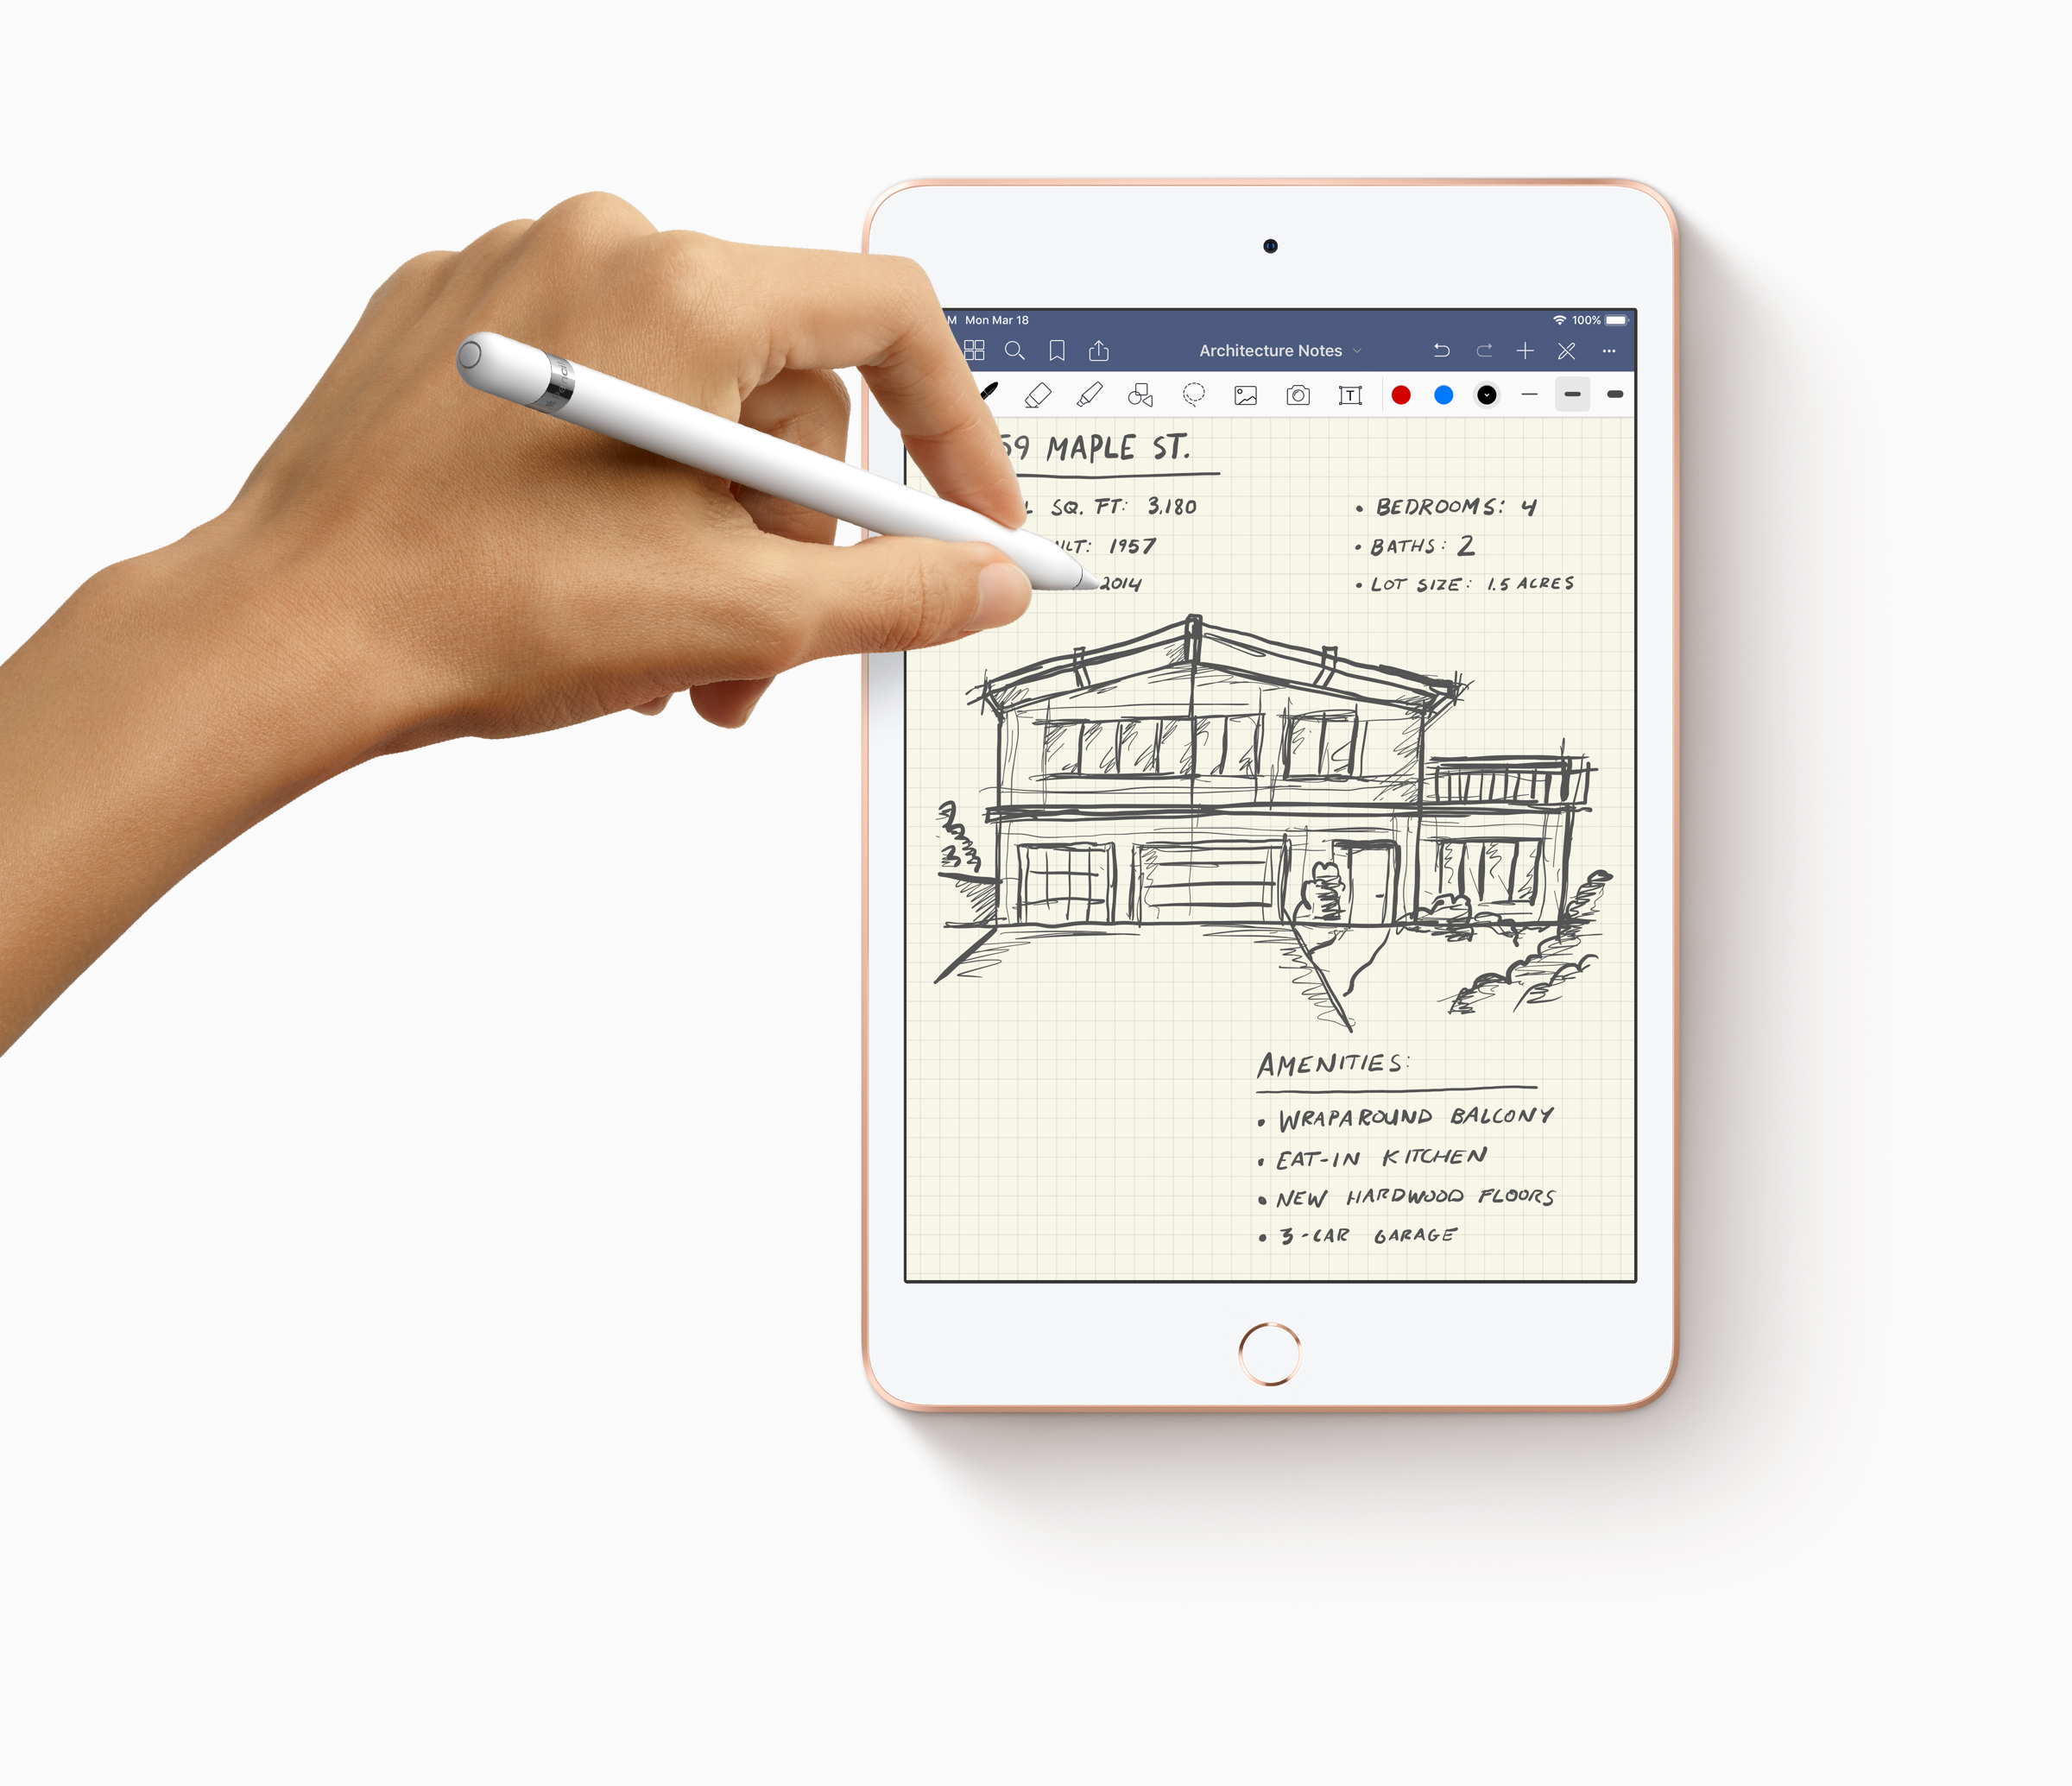
\includegraphics[width=40mm]{images/ipadmini.jpg}}
                         \end{center} \caption{iPad}
\end{minipage} \begin{minipage}{0.5\hsize}
                   \begin{center} {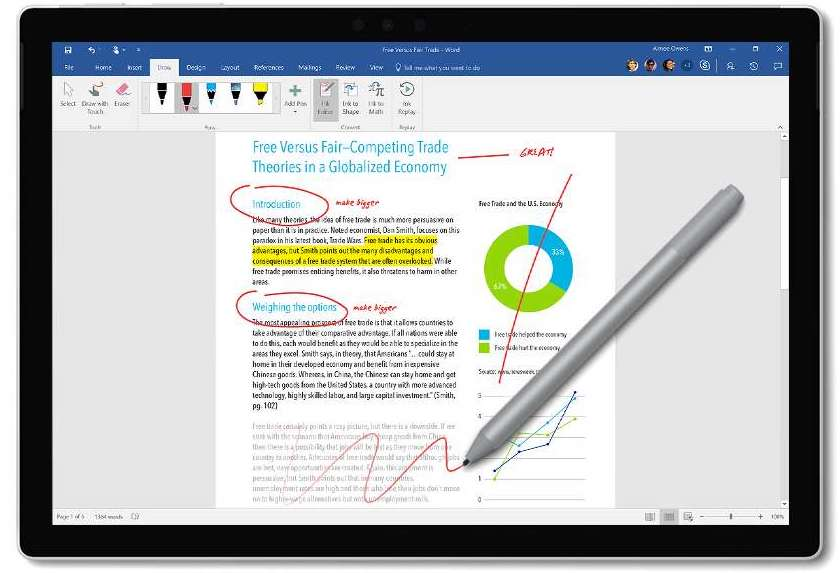
\includegraphics[width=40mm]{images/surface.jpg}}
                   \end{center} \caption{Surface}
\end{minipage}
\end{figure}

かつてはノートやスケッチブック等の紙の上で記録されていた手書きメモだが、タッチパネルやスタイラスペン等のインターフェースを備えたデバイスの普及に伴い、
計算機上で手書きメモを取ることが一般化してきた。
手書きメモやイラストを計算機の上で描く場合、マウスやトラックパッド等のポインティングデバイスではなく、
ペンインターフェースが好ましいとされるが、iOS\footnote{https://www.apple.com/jp/ios/}やWindows\footnote{https://www.microsoft.com/ja-jp/windows}、
ChromeOS\footnote{https://www.google.com/chromebook/}等の主要なプラットフォームで
スタイラスペンを備えた機種が充実しているため手書きでメモやイラストを描く環境は充分に整っている。

\section{計算機上の手書きメモ・イラスト}
計算機上でメモやイラストを作成する場合、以下のような編集支援機能を利用することができる。
\begin{itemize}
    \item コピーやペースト
    \item UndoやRedo
    \item オブジェクトの移動や変形
    \item 複数のレイヤーの合成
\end{itemize}
これらの機能は紙という物理的なメディアの上では実現不可能であったが、計算機の進化によって大抵のアプリケーションに搭載されるようになったため、
より便利に手書きのメモやイラストを作成することができるようになった。

\section{手書きデータを表現する画像ファイルフォーマット}
手書きのメモを作成する段階では計算機による便利な編集支援機能を利用できるようになったが、それを保存するファイルのフォーマットの機能は大きく制限されている。
一般的に出力先としてJPEGやPNG等のビットマップ画像が用いられているが、この種のフォーマットはレイヤーや編集履歴等の構造は保持されず、
描いたもの全てがピクセルの集合として統合・変換されるほか、一部のメタデータを除いて基本的にピクセル以外の情報を保存することができないため、紙と比較して本質的に進歩していない。
そのため画像ファイルを参照するには保存するディレクトリを予め取り決めたり、タイムスタンプを頼りに時系列順でソートしたりと、紙の上で記録していたときの不便さをそのまま引き継いでしまっている。

\section{手書きデータを扱う既存のシステム}

\subsection{デジタルペン}

\subsubsection{Anoto}

\begin{figure}[htbp] \begin{minipage}{0.5\hsize}
                         \begin{center} \fbox{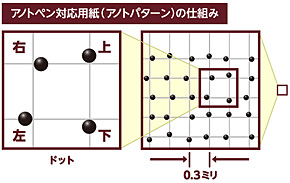
\includegraphics[width=50mm]{images/anoto1.jpg}}
                         \end{center} \caption{Anotoパターン} \label{fig:anoto1}
\end{minipage} \begin{minipage}{0.5\hsize}
                   \begin{center} \fbox{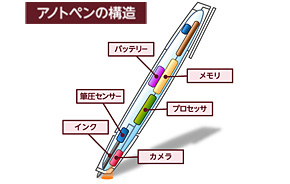
\includegraphics[width=50mm]{images/anoto2.jpg}}
                   \end{center} \caption{専用のペン} \label{fig:anoto2}
\end{minipage}
\end{figure}

Anotoによるデジタルペンは、Anotoパターンと呼ばれる微細なドットが印刷された専用の用紙に、カメラを内蔵したペンで記入することにより手書き入力をデータ化するシステムである。
専用の紙とペン以外に特殊なタブレット機器や読み取り装置を必要としないが、あくまで物理的な紙の上に記入しているためUndoやRedo等の計算機による編集支援機能は利用できない。

\subsection{メモアプリケーション}
手書きデータを効率よくメモとして扱えるようにしたシステムを解説する。

\subsubsection{iOSのメモ}

\begin{figure}[htbp]
    \begin{center}
        \fbox {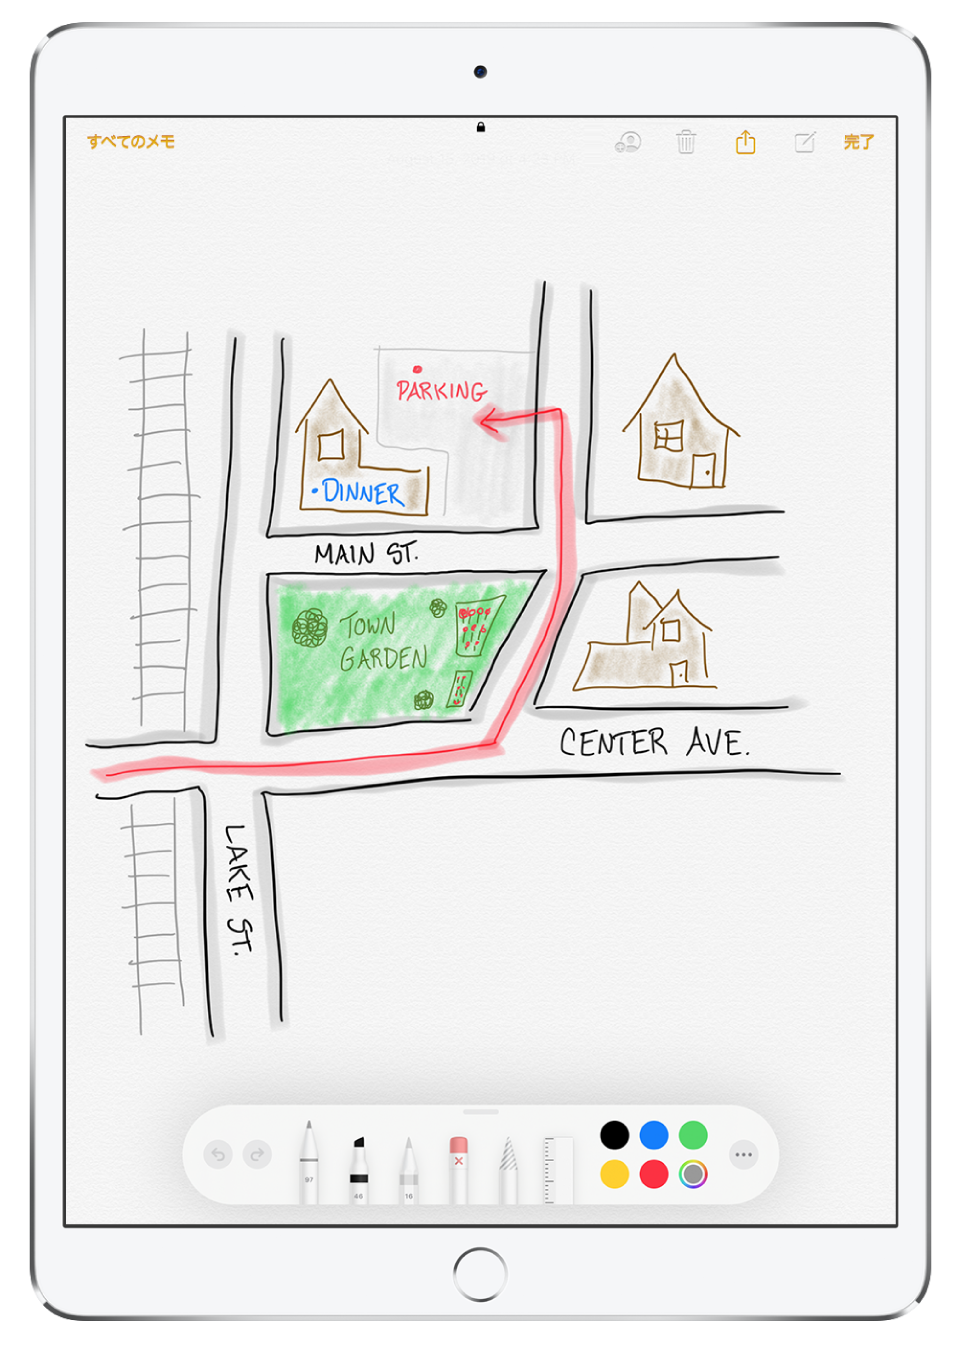
\includegraphics[width=50mm]{images/applememo.png}} \end{center}
    \caption{iOSのメモ}
\end{figure}

AppleのiPadにはメモアプリケーションが標準でインストールされており、指やApple Pencilを用いて素早く手書きメモを取ることを可能で、
さらにUndoやRedo等の編集支援機能を備えている。一方で描いた手書きメモは画像として保存されるのみで、
後から検索する手立てがなく、ファイル名の規則を決めたり保存先フォルダを分ける等の工夫が運用上必要とされる。

\subsubsection{Evernote}

\begin{figure}[htbp]
    \begin{center}
        \fbox {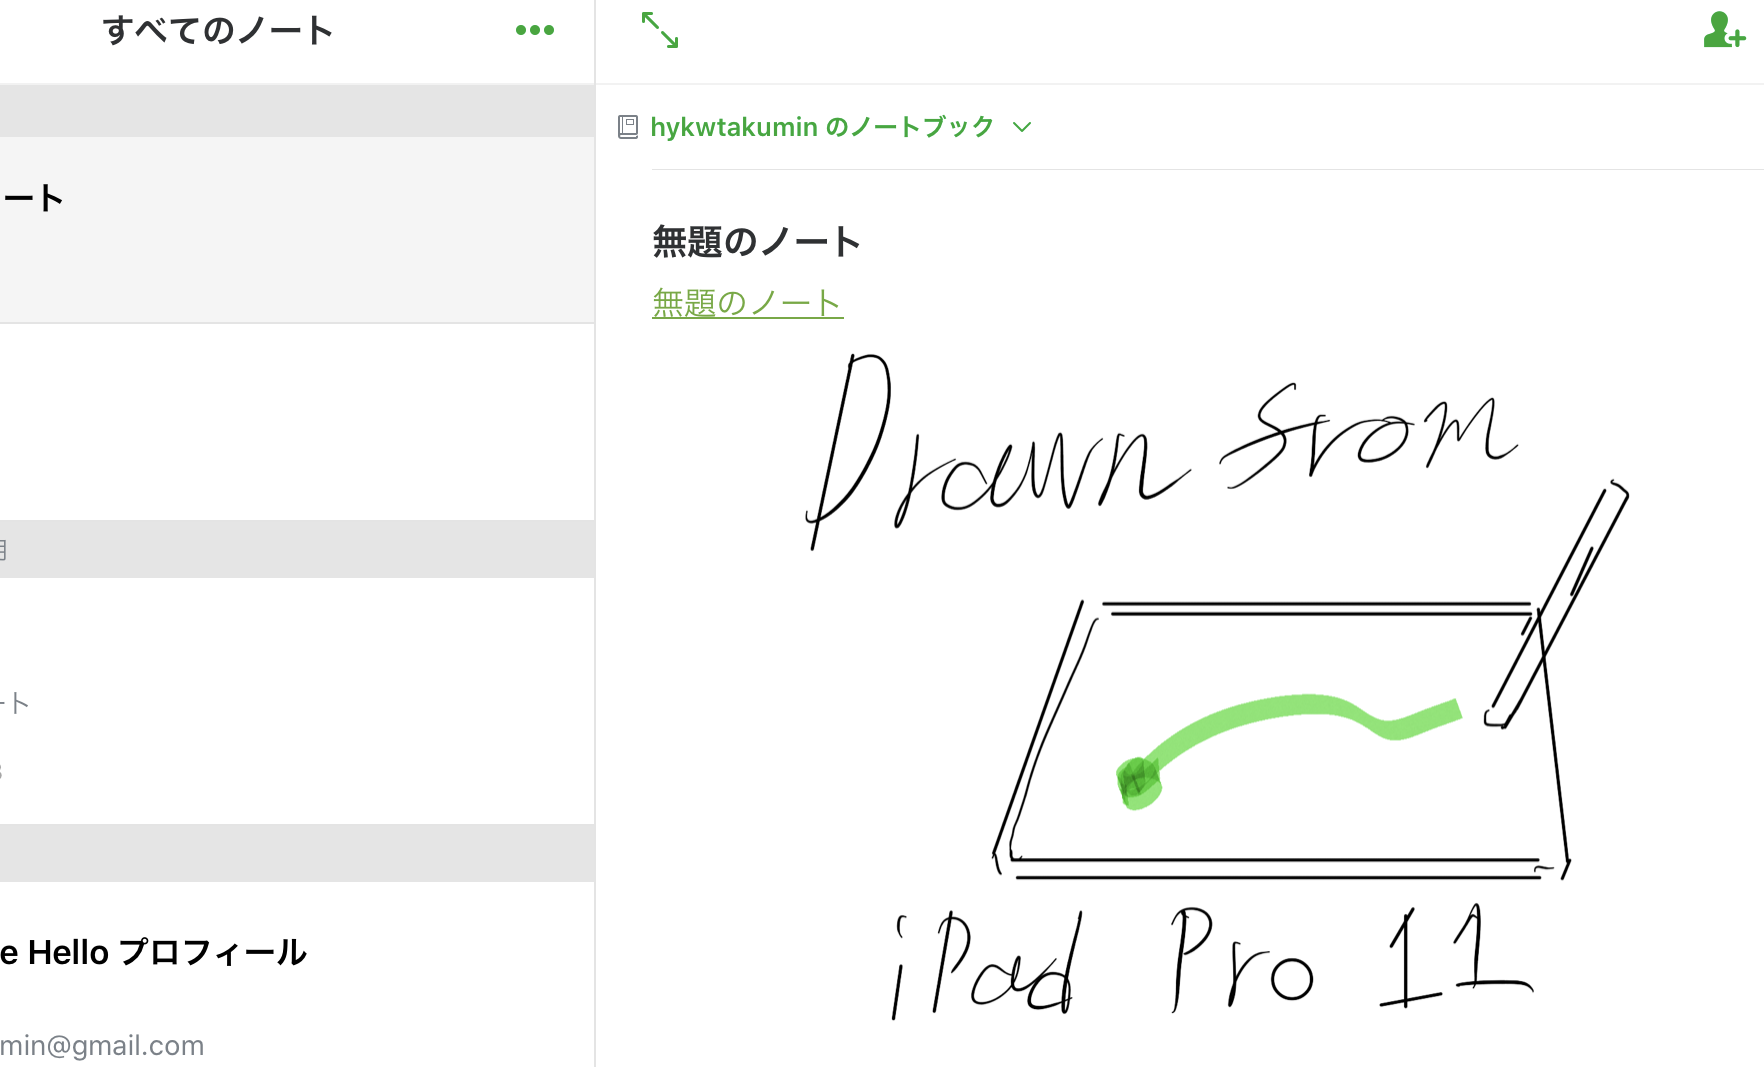
\includegraphics[width=90mm]{images/evernote.png}} \end{center}
    \caption{Evernoteによる手書きメモ}
\end{figure}

Evernote Corporationが開発するEvernoteは指やスタイラスペンで手書きのメモやスケッチを記録することができる。
手書きの文字を認識することで後からテキストによって検索する機能を備えているが、これは手書きメモをテキストに変換することで実現しているため、
図形や描いたものの形状等のグラフィカルなデータから手書きメモを参照することはできない。

\subsubsection{Google Keep}

\begin{figure}[htbp]
    \begin{center}
        \fbox{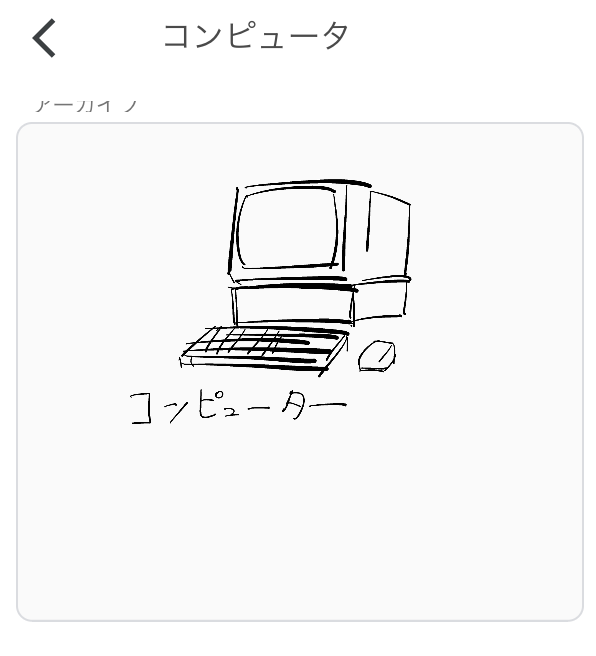
\includegraphics[width=90mm]{images/googlekeep.png}} \end{center}
    \caption{手書き文字認識によってテキスト検索から手書きメモを参照可能}
\end{figure}


Googleが開発するGoogle Keepも、Evernoteと同様にテキストによって検索することも可能である。
さらに画像や手書きメモ内にある文字を認識してテキストとして抽出する機能があるが、やはりこれも手書きメモ内の文字を
テキストに変換するというアプローチであるため、Evernoteと同様の問題を抱えている。

\subsection{イラスト投稿・共有システム}
Web上で手書きのイラストを投稿・共有可能にするシステムを解説する。
これらのシステムは基本的に完成されたアート作品を投稿するのが主な用途であり、メモを素早く記録する手段
として使われることはないが、様々な工夫によってイラストの参照や管理の問題の改善に取り組んでいる。

\subsubsection{Pixiv}

pixiv Inc.が開発するPixivでは、投稿したイラストに複数のタグを付加することができる。
また共通のタグを持つ他のイラストを関連イラストとして下部に表示する機能を備えているため、作者を横断して共通するテーマの他のイラストを参照することができる。

\begin{figure}[htbp] \begin{minipage}{0.5\hsize}
                         \begin{center} \fbox{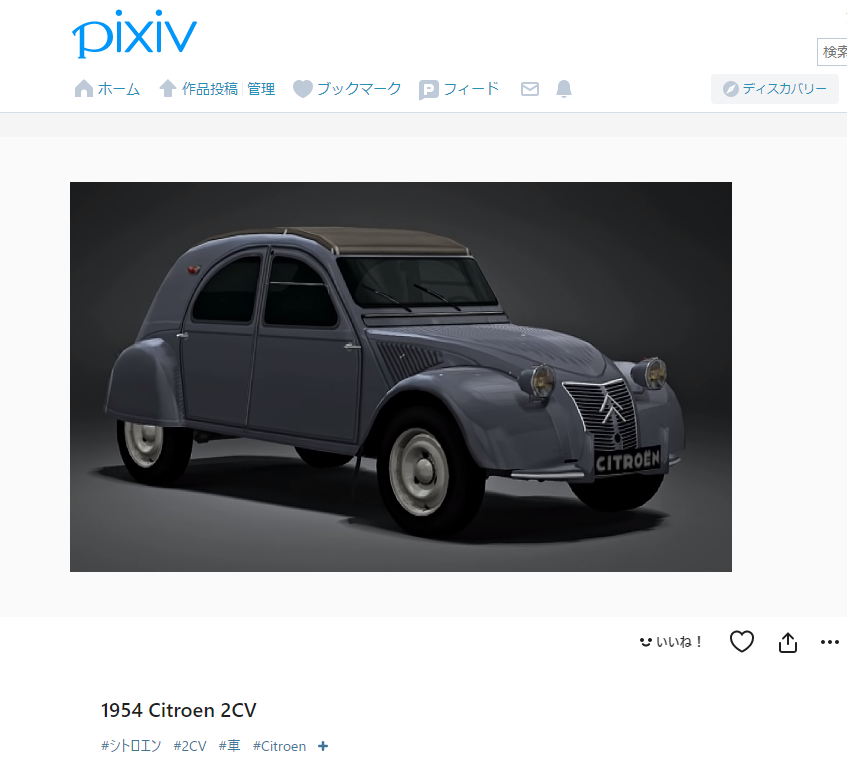
\includegraphics[width=70mm]{images/pixiv1.png}}
                         \end{center} \caption{現在閲覧している作品} \label{fig:pixiv1}
\end{minipage} \begin{minipage}{0.5\hsize}
                   \begin{center} \fbox{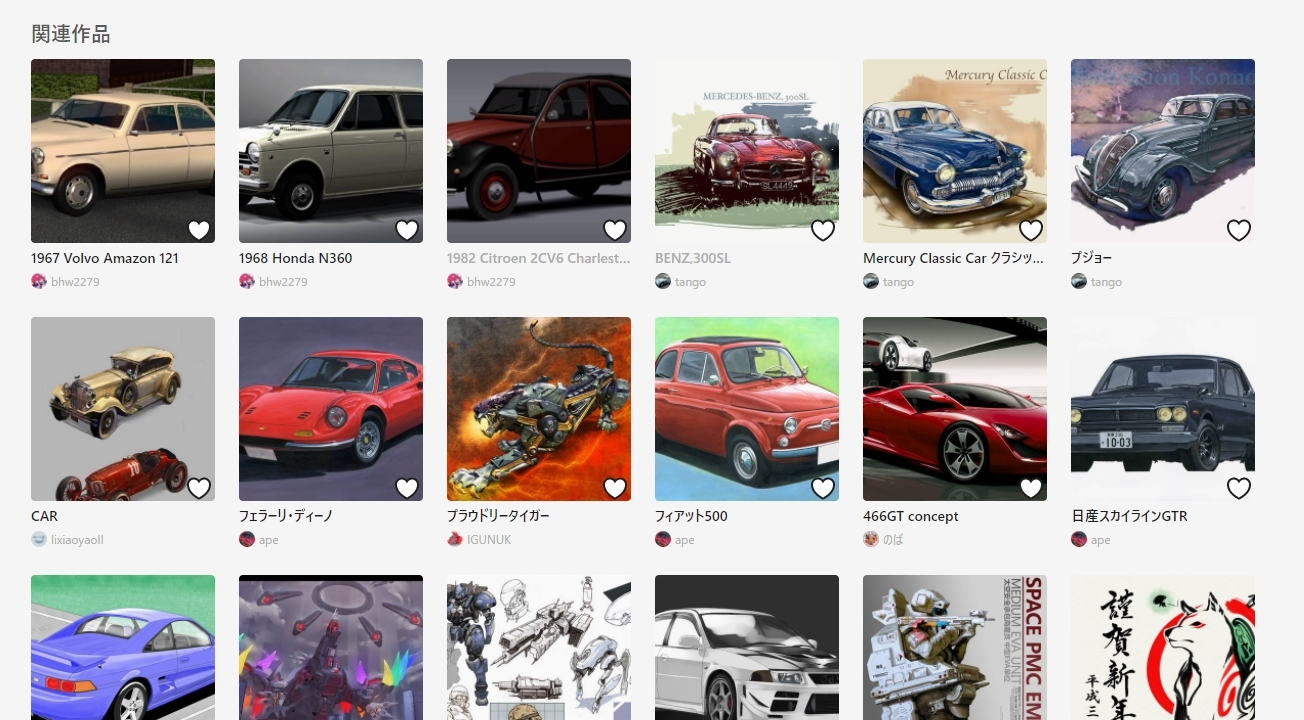
\includegraphics[width=70mm]{images/pixiv2.jpg}}
                   \end{center} \caption{閲覧中の作品に関連する作品群} \label{fig:pixiv2}
\end{minipage}
\end{figure}

\subsubsection{ニコニ・コモンズ}

ドワンゴが開発するニコニコ動画の関連サービスであるニコニ・コモンズでは、イラストも含めた素材の親子関係を記述するコンテンツツリーという機能が実装されている。
これによりある作品の元になった作品や、ある作品を元にした他の作品を参照することができる。
ただし登録は子作品の投稿者が手動で行わなければならないという制約があるため、全ての作品のコンテンツツリーが漏れなく記述されているわけではない。

\begin{figure}[htbp]
    \begin{center}
        \fbox{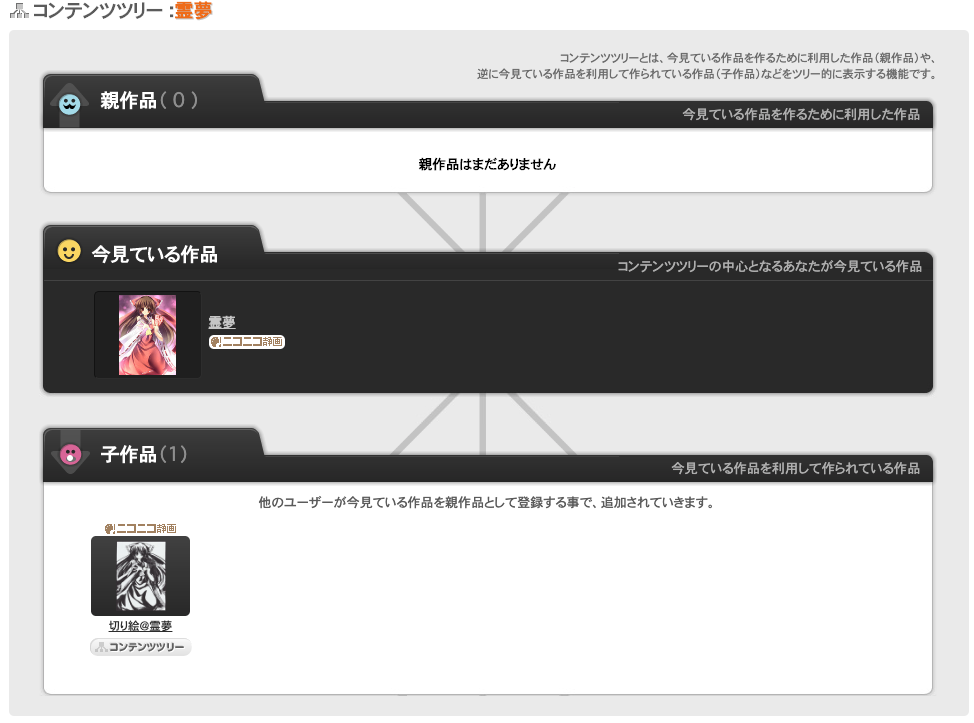
\includegraphics[width=90mm]{images/niconicommons.png}} \end{center}
    \caption{ニコニ・コモンズによって可視化されるコンテンツ間の親子関係}
\end{figure}


\section{テキストの進化}
手書きのメモやイラストと同様に紙の上で表現されていたテキストは計算機の登場により以下のような機能を獲得した。
\begin{itemize}
    \item ハイパーリンク\\
    ハイパーテキストでは文章間リンクを示すハイパーリンク機能が利用でき、関連情報への素早いアクセスが可能になった。
    \item Web\\
    インターネット技術の進化とWebの普及によって、世界中に存在する様々なドキュメントへ瞬時にアクセスすることが可能になった。
    \item 共同編集\\
    Wikiのようなコラボレーションツールによって、場所や人数に制約を受けない共同編集が可能になった。
\end{itemize}
これにより参照・管理・再利用が難しいという問題点を解決するに至った。

\section{手書きデータを扱う既存システムの問題点}
手書きデータを扱うシステムは数多く存在し活用されているものの、画像ファイルのフォーマットの機能が制限されているため、
計算機の進化によって得られる便利な機能を享受できていない。また、

\section{まとめ}
手書きメモ・イラストは広く浸透した情報の記録手法であるものの、紙というフォーマットの制約によって使い勝手が制限されている。
一方でデジタル化された手書きメモ・イラストの作成や閲覧を支援するシステムが広く利用されているが、
これらは計算機上で手書きの利用形態を再現したに過ぎず、本質的な問題は解決されていない。
次章では上記のような問題点を解決し、これまでの手書きメモ・イラストの在り方にとらわれない次世代のフォーマット「ハイパーイラスト」と、
それらを容易に管理・再利用できるシステム「手書きベースWiki」を提案する。  % 本文2
\chapter{設計}
\label{chap:sekkei}

本章ではハイパーイラストと手書きベースWikiの要件と設計について述べる。

\newpage

\section{要件}
前章で示した画像ファイルフォーマットや手書きデータを扱う既存のツールの問題点を踏まえて、本システムの要件を整理する。
\begin{enumerate}
    \item 簡単に手書きメモのメモやイラストが作成・編集できる\\
    メモを取るような気軽さで楽譜を書くことができ、新規作成/既存楽譜の編集両方を簡単に行える。
    \item 作成した手書きのメモやイラストを簡単に参照したり、再利用したりできる\\
    楽譜上の要素やテキストに対してハイパーリンクを設定でき、関連情報に素早くアクセスできる。
\end{enumerate}
これらの要件を満たすシステムは次世代の画像フォーマットであるハイパーイラストと、その作成・編集と管理をサポートする手書きベースWikiの組み合わせによって実現可能である。

\section{ハイパーイラスト}
複数の文書間の参照を示すハイパーリンクが埋め込まれた文書はハイパーテキストと定義される。
同様に本研究においてハイパーリンクが埋め込まれた手書きの図やメモをハイパーイラストと定義する。\\
この要件を満たすため、本研究におけるハイパーイラストはSVG\cite{aboutsvg}というフォーマットをベースとしている。
SVGはXML\footnote{https://www.w3.org/XML/}をベースとしており、他の画像ファイルフォーマットにはない、ハイパーイラストに適した以下のような特徴を持つ。
\begin{itemize}
    \item 構造を保持できる\\
    SVGにおいて各ストロークは独立した要素であり、個別に移動や変形等の操作が可能である。またレイヤーや書き順等の構造も保持できるため
    異なるSVGをネストして配置できるためビットマップ画像と比較して再編集・再利用が行いやすい。
    \item Web標準の技術である\\
    SVGは特定の企業の製品ではなく、その仕様は全て公開されている。また表示に特別なソフトウェアを必要とせず、
    ブラウザのみで閲覧することができる。
    \item ハイパーリンクを埋め込める\\
    XLink形式のハイパーリンクを任意の要素に埋め込むことができる。画像の中の個別の要素に対して別々のリンク
    を定義することができる。
\end{itemize}

\section{手書きベースWiki}
  % 本文3
\chapter{実装}
\label{chap:jissou}

本章では第\ref{chap:sekkei}章で述べたシステムの設計を受け、Draw Wikiの実装について述べる。

\newpage

\section{アプリケーション構成}
Draw Wikiはブラウザ上から利用できるWebアプリケーションとして実装されている。そのため
HTML5とSVG1.1に準拠したブラウザがインストールされていれば、OSやデバイスに依存せず利用することができる。
本アプリケーションの構成は以下の通りである。

\begin{figure}[htbp]
    \begin{center}
    {
\includegraphics[width=50mm]{images/testimage.png}} \end{center}
    \caption{アプリケーションの構成}
\end{figure}

\section{クライアントサイド}
実際にハイパーイラストを作成したり関連イラストを閲覧したりするクライアントサイドのプログラムはHTMLとjavascriptによって実装される。
開発にはJavascriptに変換可能な漸進的型付け言語TypeScriptを、UI操作ライブラリとしてReactをそれぞれ用いている。

\subsection{手書きデータの表現}
ブラウザに実装されているPointer-Events APIによって取得したイベントからパスのデータを生成し、描画する。
このAPIではマウスを含めてタッチやスタイラス等のあらゆるユーザー入力を透過的に扱うことができるため
あらゆる手書きデータ入力を受け付ける本システムで採用している。
このAPIはモダンなブラウザにはおおよそ搭載されているためプラットフォームを選ばずに利用できる。

\begin{figure}[htbp]
    \begin{center}
    {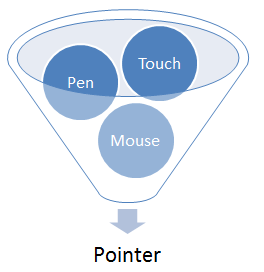
\includegraphics[width=50mm]{images/pevents.png}} \end{center}
    \caption{pointer-eventsの概要}
\end{figure}

\subsection{リンク付要素の視覚的表現}
関連イラスト表示にはリンクさせた、またはインポートしたハイパーイラストのサムネイルが表示される。
そのサムネイルを選択すると、そのハイパーイラストをリンクされている要素が強調表示される。
SVGはスタイルシートを読み込んで適用することもできるため、CSS/CSS transitionを用いて
この視覚的表現を実現している。

%\subsection{WYSIWYGエディタ}

\section{サーバーサイド}
Draw WikiはNode.js上で動作するWebアプリケーションとして実装されている。
HTTPリクエストを処理するWebアプリケーションフレームワークとしてExpressを用い、
そのホスティング環境としてBaaS(Backend-as-a-Service)の一つであるHerokuを利用している。

\subsection{ハイパーイラストのホスティング環境}
ファイルとしてのハイパーイラストはアプリケーションサーバーと異なる場所にホスティングされている。

  % 本文4
\chapter{応用例}
\label{chap:ouyou}

本章では、手書きベースWikiによって実現可能な応用例について述べる。

\newpage
\chapter{関連研究}
\label{chap:kanren}

本節では、手書きベースWikiのコンセプトや機能に関連する興味深い研究を紹介し、それらの特徴を示しつ本研究との比較を行う。
\newpage

%手書きのメモに関する先行研究は、
%個人のメモを共有可能にするもの1
%小型デバイス上でのメモ取りを支援するもの2
%3
%等数多く存在する

%アクティブリーディングにおいてもsensing grasp等が存在する4
%同様の機能をテーブルトップ上でも行うシステムが存在する56
%

\section{手書きデータをハイパーテキストとして扱うシステム}
\label{hyperillustcreators}
手書きのメモやイラスト等の画像データに対しハイパーリンクを埋めこむ機能を持つものとして
以下のようなシステムが挙げられる。

\subsection{HyperCard}
Appleによって開発されたHyperCard\footnote{http://www.apple.com/hypercard}は、マルチメディアやリンクを埋め込んだハイパーテキストのような
コンテンツを作成できるソフトウェアである。
HyperCardのコンテンツは複数のカードから構成されたスタックという形式で運用されるが、
図\ref{fig:hypercard}のように手書きの図の上にフィールドを作成し、マウスでクリックした際に
異なるカードへの移動するという処理をHyperTalkと呼ばれるスクリプト言語で記述することで
ハイパーリンクに相当する機能を実現することができる。

\paragraph*{DrawWikiとの比較}
HyperCardでは手書きの図を含むあらゆるオブジェクトに対してカード間リンクを埋めこむことができるが、
その設定にはコーディングが必要であり敷居が高い。DrawWikiは範囲選択ツールで要素を選び、リンク先のメモ・イラスト
を設定するだけで同じ操作ができるため手数が少なく、より手軽であると言える。
またカード間は自在に移動できるが異なるマシンに置かれたスタックに対してアクセスすることができない。
DrawWikiでは全てのメモ・イラストがURLを持ったハイパーテキストであるため全世界からアクセス可能である。

\begin{figure}[H]
    \centering
    \fbox{ 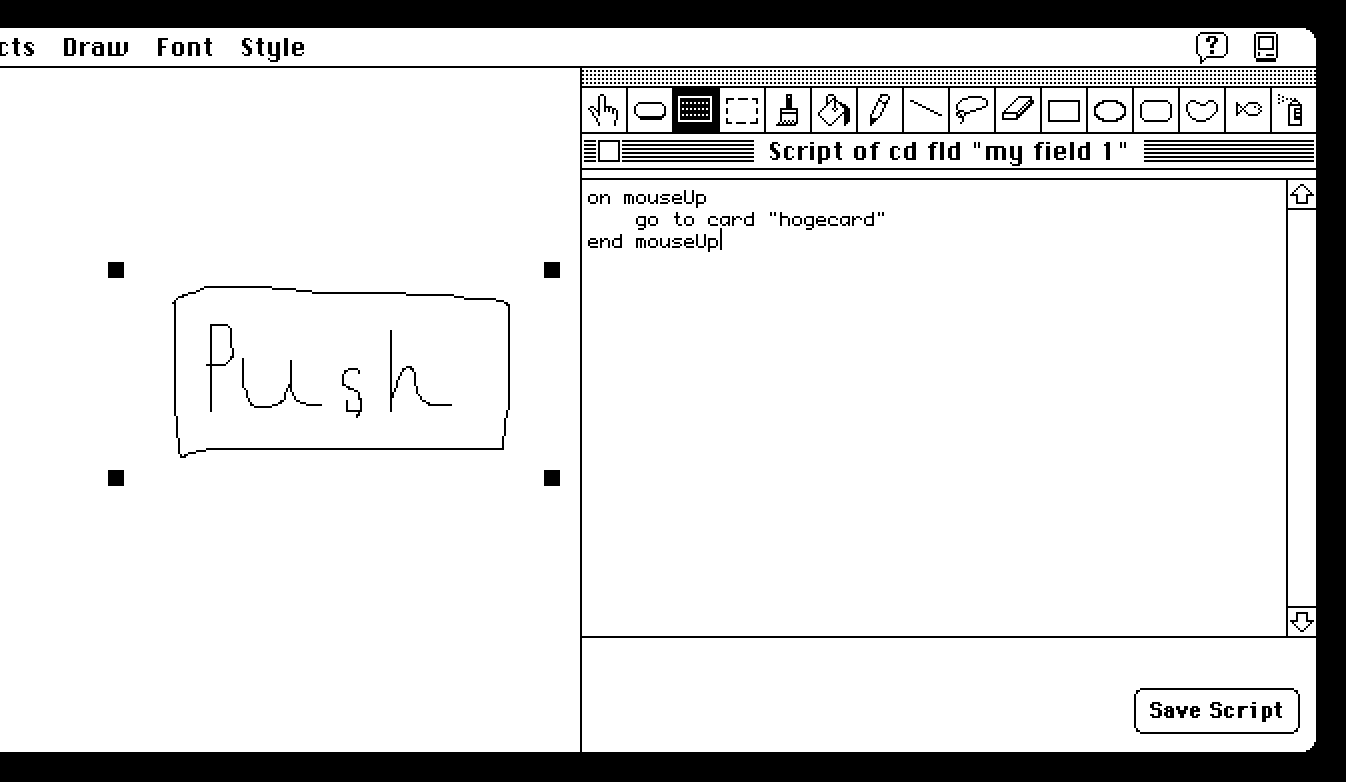
\includegraphics[width=11cm]{images/hypercard.png} }
    \caption{エミュレータ上で再現されたHyperCardの編集画面}
    \label{fig:hypercard}
\end{figure}

\subsection{Adobe Photoshop}
Adobe Systems\footnote{https://www.adobe.com/}が開発する画像編集ソフトウェアであるPhotoshop\footnote{https://www.adobe.com/jp/products/photoshop.html}には
作成した画像をHTMLファイルとして出力するオプションが存在する。設定によっては任意の領域に対してハイパーリンクを埋めこむことができる。
この時出力されるファイルは、本体となる画像とそれをオーバーレイするHTMLファイルとセットで構成される。

\paragraph*{DrawWikiとの比較}
そもそもPhotoshopはプロフェッショナル向けのツールであり、すばやく手書きメモを取るという用途に対して多機能すぎるため、大袈裟である。
また画像付きHTMLファイルとして出力した場合、各ファイルを正しい位置関係に配置したディレクトリごと配布される必要があり、
1ファイルで画像とハイパーリンクの双方を記述できるSVGと比較してポータビリティに欠ける。

\subsection{Inkscape}
The Inkscape Team\footnote{https://inkscape.org/user/teams/}によって開発されるオープンソースのベクター画像編集ソフトウェアである
Inkscape\footnote{https://inkscape.org/}はSVG画像をテキストエディタによって直接編集する機能を備える。
これにより複数の要素をグループ化し、同一のハイパーリンクを埋めこむ等の高度な操作を行うことができる。

\paragraph*{DrawWikiとの比較}
Photoshopと同様Inkscapeも手書きメモという用途に対して高機能すぎ、またSVGを直接編集するには
SVGやXMLの仕様についてよく理解している必要があるため敷居が高い。
DrawWikiではSVGの構造をユーザーが意識することなく同一の操作を実現できる。
またPhotoshopと同様サポートしている機能は画像に対するハイパーリンクの埋め込みのみで、
ホスティング等は行わない。したがって作った画像を参照可能にするためには、ユーザー自らがリンクさせる画像をサーバーに
ホスティングしなければならないため、Wikiツールとして活用するには機能不足であると言える。

\section{手書きデータによって文書の参照や管理・再利用を支援するシステム}
メモやイラストに限らず文字を書く、下線を引く、丸で囲む等の手書きデータを
文書の閲覧や検索に応用し、参照や管理・再利用に活用する試みとして以下のシステムが挙げられる。

\subsection{XLibris}
\begin{figure}[H]
    \centering
    \fbox{ 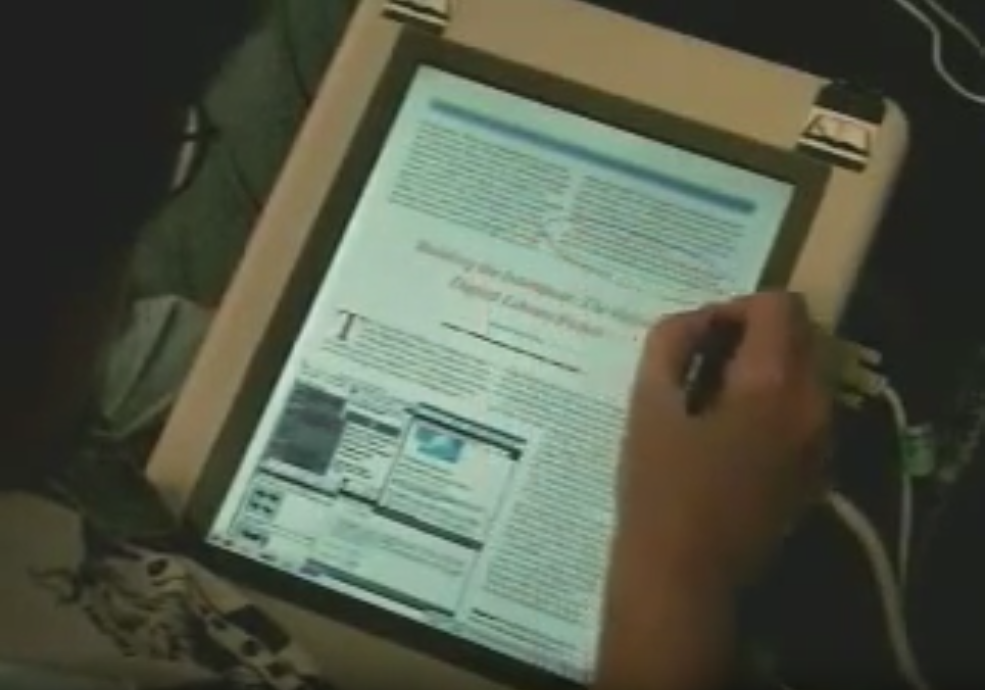
\includegraphics[width=10cm]{images/xlibris.png} }
    \caption{操作中のXLibris}
    \label{fig:xlibris}
\end{figure}
PriceらによるXLibris\cite{Price1998XLibrisTA}(図\ref{fig:xlibris})はタブレットデバイス上でActive Readingを行うことを目的としたシステムである。
スタイラスペンによって手書きの注釈やハイライトを文章中に自在に追記できるほか、
追記した部分をリンクとしてページの参照に用いたり、ハイライトされた単語や文章を検索に利用し関連資料を余白に表示する機能を備えている。

\paragraph*{DrawWikiとの比較}
メモやイラストではなく文書に追記する注釈が対象であるというコンセプトの相違があるものの、手書きの注釈がリンクとなり文書を参照しやすくなる機能や、
追記されたページを関連資料として表示する機能がActive Readingといった用途においても有用であることが示されている。

\subsection{InkSeine}
Hinckleyらによって開発されたInkSeine\cite{Hinckley2007InkSeineIS}(図\ref{inkseine})はペンインターフェースを備えたタブレットPC上での利用を想定した
Active note takingのためのシステムである。
テキスト入力も手書き文字認識によって行われる等、キーボードを使わずにペンのみで操作が完結するようUIが設計されている。
また入力した手書き文字をWebページやローカルファイルの検索に活用したり、検索結果のスクリーンショットをリンクと共にキャンバスに貼り付ける等の機能を備えており、
積極的な情報の再利用を実現している。

\paragraph*{DrawWikiとの比較}
手書きの文字を認識し、検索結果をリンクと共にノートに配置するという機能によって
ペンベースの個人用電子スクラップブックとして活用することは可能であるものの、
Wikiシステムとしての活用は想定されておらず、作成したノートのURLによる共有や
共同編集等の機能はない。

\begin{figure}[H]
    \centering
    \fbox{ 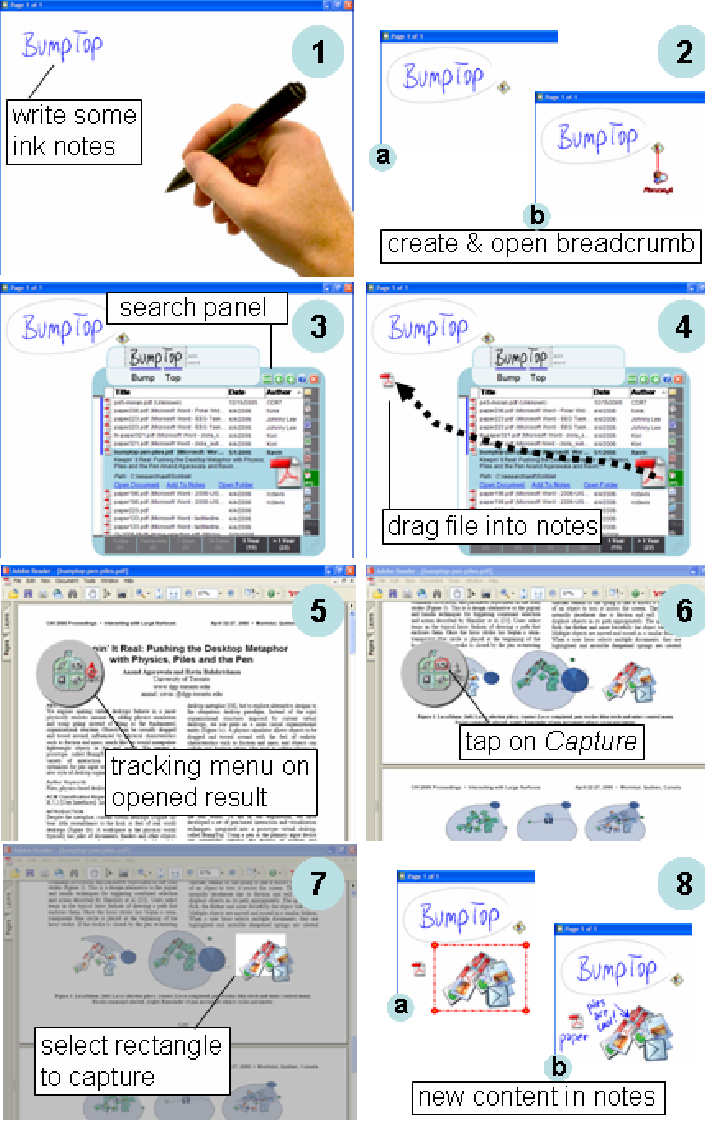
\includegraphics[width=10cm]{images/inkseine.png} }
    \caption{InkSeineの操作画面}
    \label{inkseine}
\end{figure}

\section{手書きスケッチをプロトタイピングに応用するシステム}
アプリケーションやWebサイトのUIをデザインする初期の段階ではスケッチがよく利用される\cite{Newman2000SitemapsSA}。
スケッチとしての手書きデータをそのプロトタイピングに取り入れる試みとして以下のシステムが挙げられる。

\subsection{DENIM}
\label{denim}

\begin{figure}[H] \begin{minipage}{0.5\hsize}
                         \begin{center} \fbox {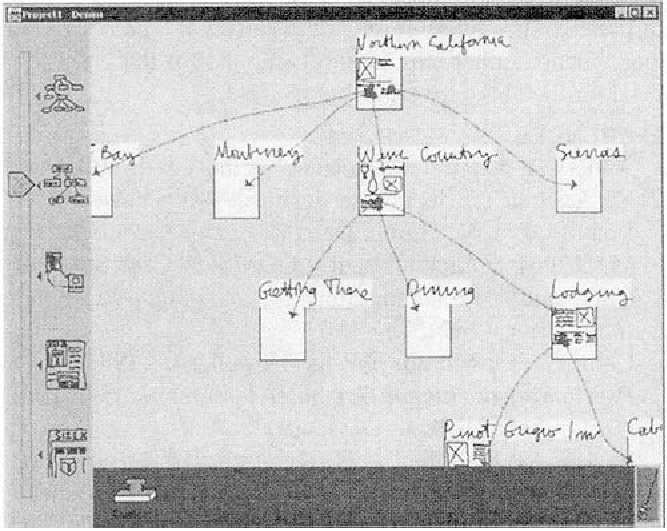
\includegraphics[width=70mm]{images/denim1.png}}
                         \end{center} \caption{DENIMの画面} \label{fig:denim1}
\end{minipage} \begin{minipage}{0.5\hsize}
                   \begin{center} \fbox {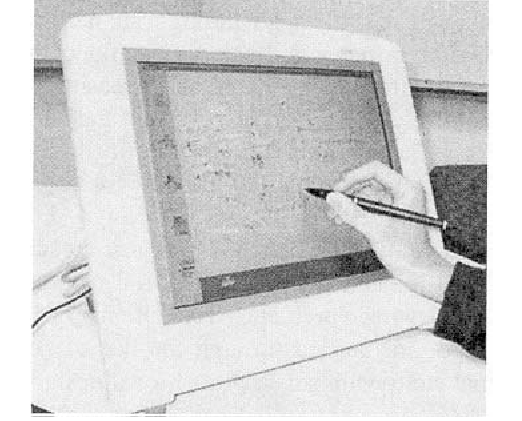
\includegraphics[width=70mm]{images/denim2.png}}
                   \end{center} \caption{操作を行うタブレット機器} \label{fig:denim2}
\end{minipage}
\end{figure}

Linらはタブレットからのスケッチを元にWebサイトのデザインやナビゲーションの設計の支援を行うシステムDENIMを開発した\cite{Lin2000DENIMFA}(図\ref{fig:denim1})。
図\ref{fig:denim2}のようなタブレット機器から操作するよう設計されており、Webページを手書きでスケッチし、それらを線で結ぶことでリンクによるナビゲーションを再現した
Webサイトのモックアップを作成することができる。またWebページの細部のデザインといった小さな視点から、複数のページ間の繋がりを俯瞰的に確認するという大きな視点までを
柔軟にカバーするために、スケッチ用キャンバスの横に視点レベルを変更可能なレンジバーが備えられており、ズーミングインターフェースの知見が取り入れられているのが
特徴である。

\subsection{SILK}
\label{silk}

\begin{figure}[H]
    \centering
    \fbox{ 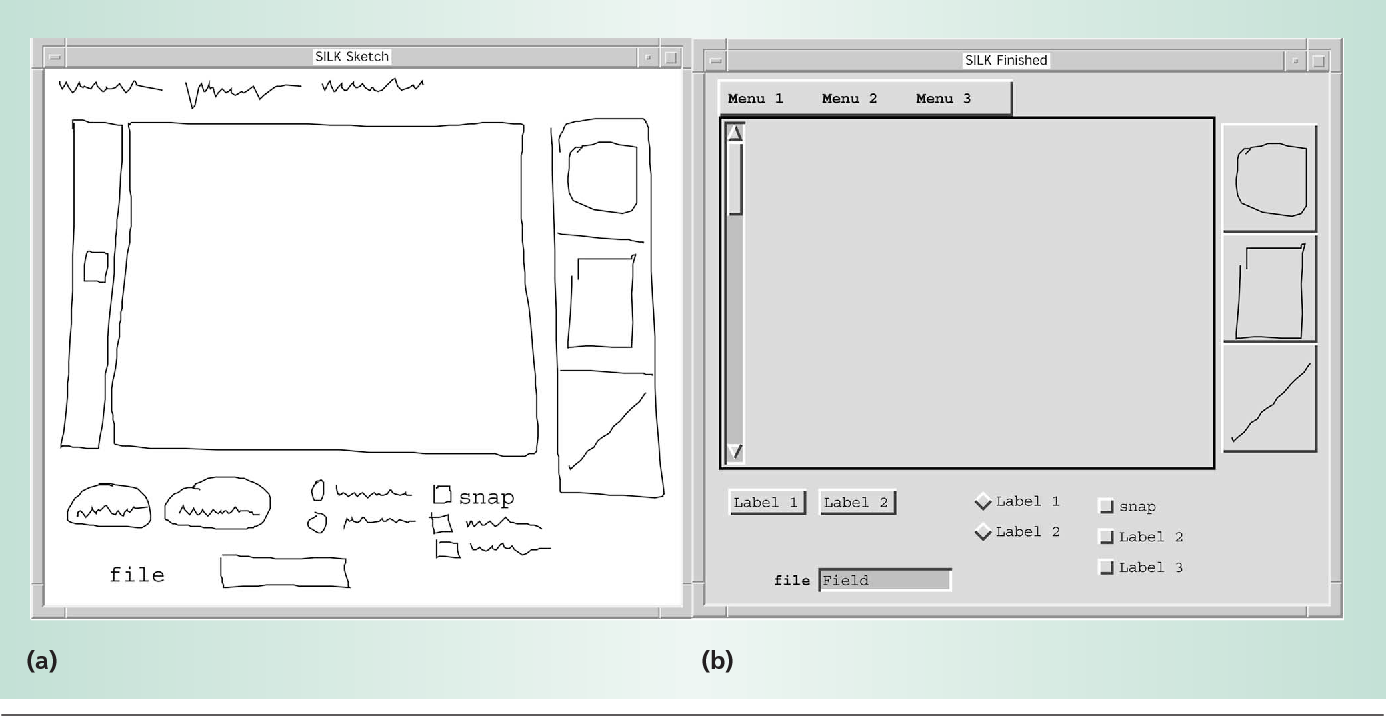
\includegraphics[width=10cm]{images/silk.png} }
    \caption{SILKの画面}
    \label{fig:silk}
\end{figure}

Landayらはスタイラスから入力した手書きデータから実際に動作するGUIを構築するSILK(Sketching Interfaces Like Krazy)というシステムを実装した
\cite{Landay2001SketchingIT}(図\ref{fig:silk})。
このシステムは手書きデータの形状からボタンやフォーム等のUIコンポーネントを類推し、配置することで動作可能なソフトウェアのプロトタイプを
構築することができる。

\paragraph*{DrawWikiとの比較}
いずれのシステム(第\ref{denim}節、第\ref{silk}節)も、ラフスケッチの段階である程度のインタラクションを再現するプロトタイプを作成可能なことが
デザインを行う上で役立つことを示している。DrawWikiはデザインを専門とするツールではないが、手書きスケッチの内部へのリンク埋め込みや、
リンク先画像のダイアログ表示といった機能を用いることで第\ref{drawiki:mockup}節のように「インタラクションを伴うプロトタイプ」として応用することができる。
したがってDrawWikiはデザインの分野においても応用可能なツールであると言える。
%さらにDrawWikiは本来のWikiとしての機能も備えているため、書き捨てることが一般的だったラフスケッチをリンクによって参照・再利用可能な活きたナレッジ
%として活用することができる。

\section{手書きスケッチの中の要素に注釈を埋め込めるシステム}
手書きのスケッチの内部に、手書きのメモ・イラストや画像、音声等のメディアを注釈として埋めこむシステムとして
以下が挙げられる。

\subsection{SketchComm}
\label{sketchcomm}

\begin{figure}[H] \begin{minipage}{0.5\hsize}
                      \begin{center} \fbox {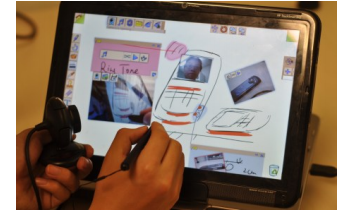
\includegraphics[width=70mm]{images/sketchcomm1.png}}
                      \end{center} \caption{} \label{fig:sketchcomm1}
\end{minipage} \begin{minipage}{0.5\hsize}
                   \begin{center} \fbox {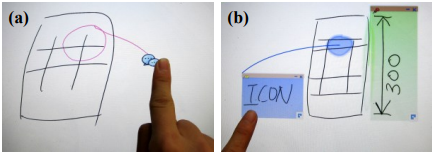
\includegraphics[width=70mm]{images/sketchcomm2.png}}
                   \end{center} \caption{} \label{fig:sketchcomm2}
\end{minipage}
\end{figure}
LiらによるSketchComm\cite{Li2012SketchCommAT}はアイデアに関するスケッチが非同期的にレビューされることを念頭に置いて設計されたシステムである(図\ref{fig:sketchcomm1})。
対面によるコミュニケーションを伴う同期的なレビューと異なり、非同期的なレビューではコンテキストが欠落する恐れがあるため、
それを補うために注釈やコメント、音声データ等をスケッチの内部に埋め込むことができる(図\ref{fig:sketchcomm2})。
これらのコンテンツはキャンバスを専有しないよう必要に応じて表示・非表示を切り替えられる。このシステムを用いた評価実験を行ったところ、「注釈を活用することでスケッチの視認性を
確保しながらも必要な情報は適宜参照できること」が実験に参加したデザイナーから高く評価されていた。またOneNote\footnote{https://www.onenote.com/}等の既存のシステム
との比較も行われており、 「同じコンセプトを表現する場合、注釈が利用できないOneNoteでは多くの情報をキャンバスに描かなければならないためスケッチが見づらくなった」「SketchCommの方がOneNoteよりも
少ない労力で多くを表現できる」という評価がなされている。

\paragraph*{DrawWikiとの比較}
DrawWikiが手書きメモ・イラストの中に埋めこむのはハイパーリンク(URL)であるが、クリックすると即座に遷移するのではなく
リンク先の画像がダイアログで表示されるため、第\ref{drawiki:mockup}節や第\ref{drawiki:zukai}節のように「表示/非表示を切り替え可能な注釈」として活用することができる。
スケッチの内部に関連する情報をあわせて保存できることがコンセプトの理解を助けることをこの研究は示しており、この機能はWikiシステムにおいても有効であると考えられる。
\chapter{考察}
\label{chap:kosatsu}

本章では、手書きベースWikiシステムの自身の運用経験や利用者の意見をまとめ、諸問題や研究の重要性・発展性について述べる。

\newpage

\section{評価}
本節では、
\begin{itemize}
    \item 筆者の運用経験
    \item ユーザーからのフィードバック
    \item 各種展示発表でのフィードバック
\end{itemize}
をまとめる。

\subsection{筆者の運用経験}

\subsection{ユーザーインタビュー}

\subsection{意見・感想}

\subsection{問題点}
以下のような問題点が明らかになった。


\section{考察}

\subsection{設計の妥当性}

\subsection{解決すべき課題}

\subsection{手書きメモ・イラストの問題点の検証}


\chapter{結論}
\label{chap:ketsuron}

本章では本研究を総括する。

\newpage

\section{研究の成果}
本研究では、ハイパーリンクを内蔵した次世代の手書きデータ記述形式「ハイパーイラスト」と、それをコンテンツとして扱うWikiシステム「手書きベースWiki」の提案を行った。

まず第\ref{chap:haikei}章において、既存の手書きメモ・イラストの問題点をテキストの進化と比較しながら分析した。
計算機上で手書きメモ・イラストを扱う既存システムの現状をとりあげ、計算機が普及した現在も根本的に解決されていないことを示した。

第\ref{chap:sekkei}章では、第\ref{chap:haikei}章で述べた手書きメモの問題点に対する解決方法として「手書きベースWiki」を提案した。
また、「手書きベースWiki」のプロトタイプとして実装した「DrawWiki」の機能を使い方と共に解説した。

第\ref{chap:zissou}章では、「DrawWiki」のアプリケーション構成と詳細な実装について述べた。

第\ref{chap:riyourei}章では、「DrawWiki」によって実現可能な利用例を紹介した。

第\ref{chap:kanren}章では、本研究に関連する研究を紹介し、それぞれのアプローチの特徴と問題点を分析し、本研究との比較検討を行った。

第\ref{chap:kosatsu}章では、ユーザーからのフィードバックや筆者による運用経験をもとに本研究の有効性と問題点を分析した。

\section{総括}
本研究では手書きのメモやイラストの中に自在にハイパーリンクを埋め込み、それらをナレッジとして扱える「手書きベースWiki」の開発を行った。
「手書きベースWiki」はハイパーリンクやWiki等の技術の組み合わせによって、参照や管理、再利用が難しいといった手書きのメモ・イラスト問題点を解決した。
また新しい活用法を実現した。
さらにテキストベースWikiに対しても優れた点があることを示した。
今後は第\ref{chap:kosatsu}章で述べた問題点を受け、システムを改善していく。

\begin{acknowledgment}

慶應義塾大学環境情報学部 増井俊之教授には学部から5年間の長きに渡りご指導を賜りました。深く感謝いたします。また、本研究の副査としてご意見、ご助言を頂きました中西泰人教授、武田圭史教授に感謝いたします。
また自身の研究について幅広い議論をしていただいた政策・メディア研究科博士課程の田中優氏、大和比呂志氏を初め、様々な形でアドバイスをくださった増井俊之研究会OB諸氏に感謝いたします。
\\
\begin{flushright}
    2020年1月 慶應義塾大学 政策・メディア研究科 修士2年 早川匠
\end{flushright}

\end{acknowledgment}
  % 謝辞。要独自コマンド、include先参照のこと
\include{91_bibliography}  % 参考文献。要独自コマンド、include先参照のこと
\appendix

%\include{92_appendix}    % 付録、インタビュー項目等はここに配置する?

\end{document}
